\section{Introduction}


\begin{figure}[!t]
  \centering
  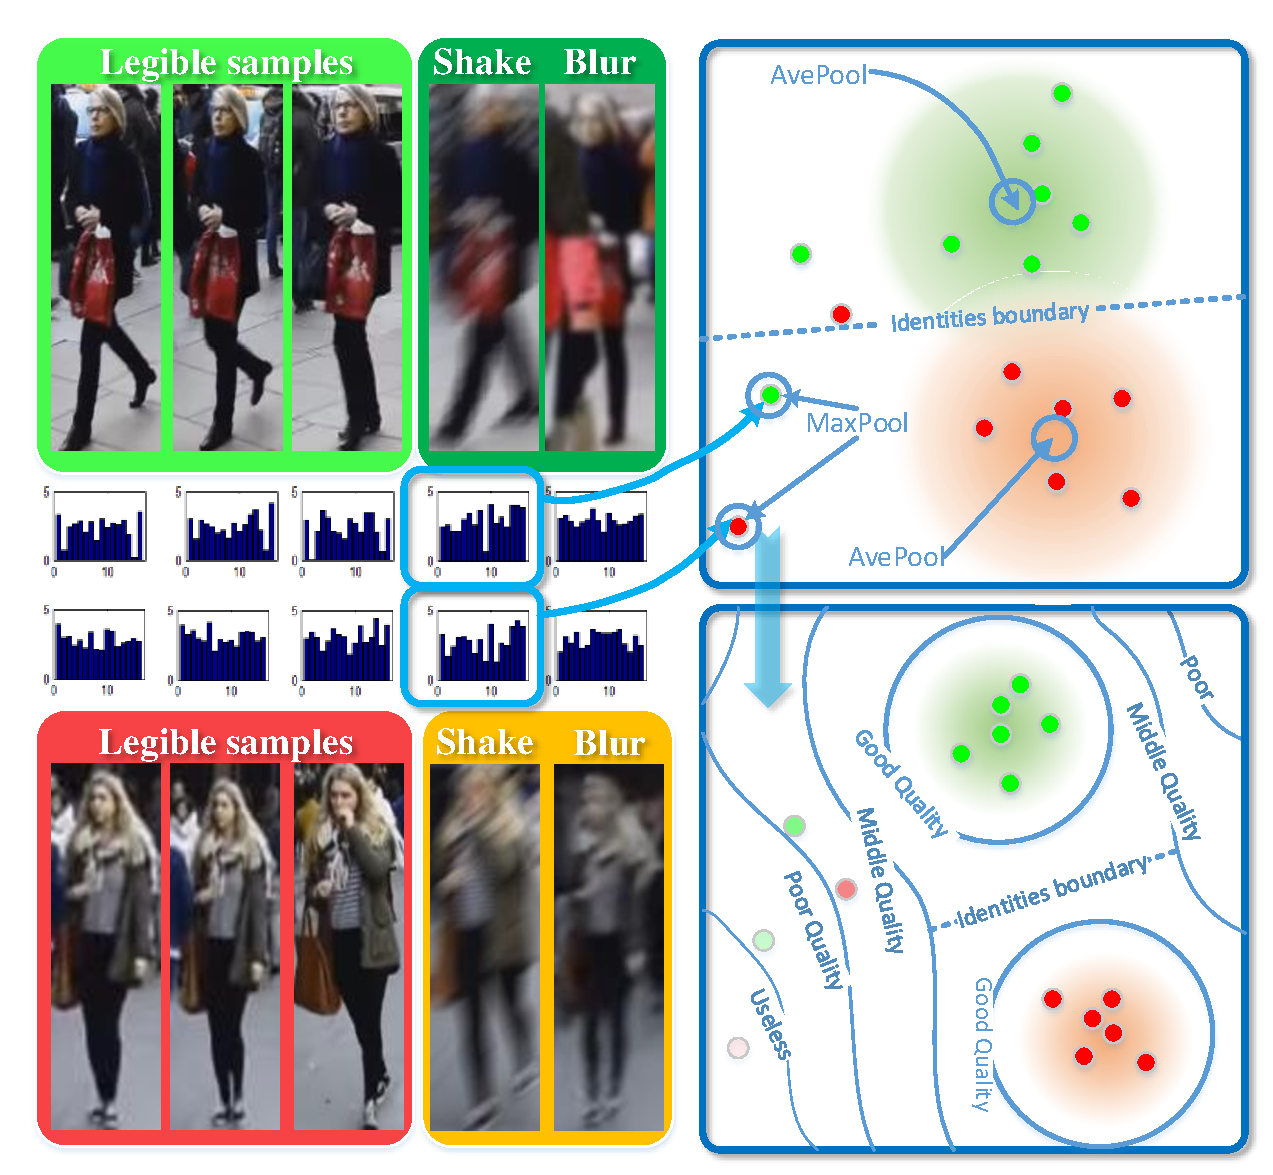
\includegraphics[width=8cm]{figure_first.pdf}
  \caption{Illustration of our motivation, best viewed in color. \emph{\textbf{Left column:}} A classical puzzle in set-to-set recognition. Both set A (upper) and B (lower) contain noisy image samples caused by shake and blur. Their features (shown by histograms in middle row) are more similar to samples in other class than the inner class.  \emph{\textbf{Right column:}} Distributions and samples of two identities in hyperspace. Top: Due to the noisy, variances of two identities are large and they both have hard negative samples. Bottom: Quality aware network (QAN) weaken the noisy samples and narrow down identities' variances, which makes them more discriminative.}
  \label{fig:fig1}
\end{figure}

Face verification \cite{sun2014deep1,learnedlabeled,sun2014deep,taigman2014deepface,schroff2015facenet} and person re-identification \cite{gong2014person,farenzena2010person,zheng2011person,li2014deepreid} have been well studied and widely used in computer vision applications such as financial identity authentication and video surveillance. Both the two tasks need to measure the distance between two face or person images. Such tasks can be naturally formalized as a metric learning problem, where the distance of images from the same identity should be smaller than that from different identities. Built on large scale training data, convolutional neural networks and carefully designed optimization criterion, current methods can achieve promising performance on standard benchmarks, but may still fail due to appearance variations caused by large pose or illumination.

In practical applications, instead of one single image, a set of images for each identity can always be collected. For example, the image set of one identity can be sampled from the trajectory of the face or person in videos. Images in a set can be complementary to each other, so that they provide more information than a single image, such as images from different poses. The direct way to aggregate identity information from all images in a set can be simply max/average pooling appearance features of all images. However, one problem in this pooling is that some images in the set may be not suitable for recognition. As shown in Figure~\ref{fig:fig1}, both sets from left-top and left-bottom hold noisy images caused by shake or blur. If the noisy images are treated equally and max/average pooling is used to aggregate all images' features, the noisy images will mislead the final representation.

In this paper, in order to be robust to images with poor quality as described above and simultaneously use the rich information provided by the other images, our basic idea is that each image can have a quality score in aggregation. For that, we propose a quality aware network (QAN), which has two branches and then aggregated together. The first branch named \emph{feature generation part} extracts the feature embedding for each image, and the other branch named \emph{quality generation part} predicts quality score for each image. Features of images in the whole set are then aggregated by the final \emph{set pooling unit} according to their quality. 

A good property of our approach is that we do not supervise the  model by any explicit annotations of the quality. The network can automatically assign low quality scores to images with poor quality in order to keep the final feature embedding useful in set-to-set recognition. To implement that, an elaborate model is designed in which embedding branch and score generation branch can be jointly trained through optimization of the final embedding.  Specially in this paper, we use the joint triplet and softmax loss on top of image sets. The designed gradient of image set pooling unit ensures the correctness of this automatic process. 

Experiments indicate that the predicted quality score is correlated with the quality annotated by human, and the predicted quality score performs better than human in recognition. In this paper, we show the applications of the proposed method on both person re-identification and face verification. For person re-identification task, the proposed quality aware network improves top-1 matching rates over the baseline by 14.6\% on iLIDS-VID  and 9.0\% on PRID2011. For face verification, the proposed method reduces 15.6\% and 29.32\% miss ratio  when the false positive rate is 0.001 on YouTube Face and IJB-A benchmarks.

The main contributions of the paper are summarized as follows.
\begin{itemize}
\item The proposed quality aware network automatically generates quality scores for each image in a set and leads to better representation for set-to-set recognition.

\item We design an end-to-end training strategy and demonstrate that the quality generation part and feature generation part benefit from each other during back propagation.

%\item An adaptive cascade structure is designed to learn a better quality generator. It can adapt different classifiers to the images with different qualities.

\item  Quality learnt by QAN is better than quality estimated by human and we achieves new state-of-the-art performance on four benchmarks for person re-identification and face verification.
\end{itemize}

